\documentclass[11pt,a4paper]{article}

\usepackage{amsmath,amssymb}
\usepackage{geometry}
\usepackage{hyperref}
\usepackage{booktabs}
\usepackage{graphicx}
\usepackage{xcolor}
\usepackage{parskip}
\usepackage{microtype}

\geometry{margin=2.5cm}

\hypersetup{
  colorlinks=true,
  linkcolor=blue!60!black,
  urlcolor=blue!60!black,
  citecolor=blue!60!black
}

\graphicspath{{figures/}}

\title{\textbf{Rocket Aerodynamics}\\
\large Model Description}
\author{}
\date{}

\begin{document}
\maketitle
\tableofcontents
\newpage

% =============================================================================
\section{Body-Fixed Coordinate Frame}
% =============================================================================

All aerodynamic forces and moments are expressed in the \textbf{body-fixed coordinate frame}, attached to the rocket and moving with it. The frame is defined as follows:

\begin{itemize}
  \item \textbf{Origin} --- at the center of mass of the rocket.
  \item \textbf{$X_{BF}$ axis} --- along the longitudinal axis of the rocket, pointing from the tail toward the nose.
  \item \textbf{$Y_{BF}$ axis} --- orthogonal to $X_B$, lying in the plane of symmetry of the rocket.
  \item \textbf{$Z_{BF}$ axis} --- perpendicular to the plane of motion, completing the right-handed triad.
\end{itemize}

For the 2D case, the pitch angle $\vartheta$ is measured from the vertical (inertial) axis to the rocket's $X_B$ axis, with \textbf{positive values corresponding to a rightward tilt}.

\begin{figure}[h]
  \centering
  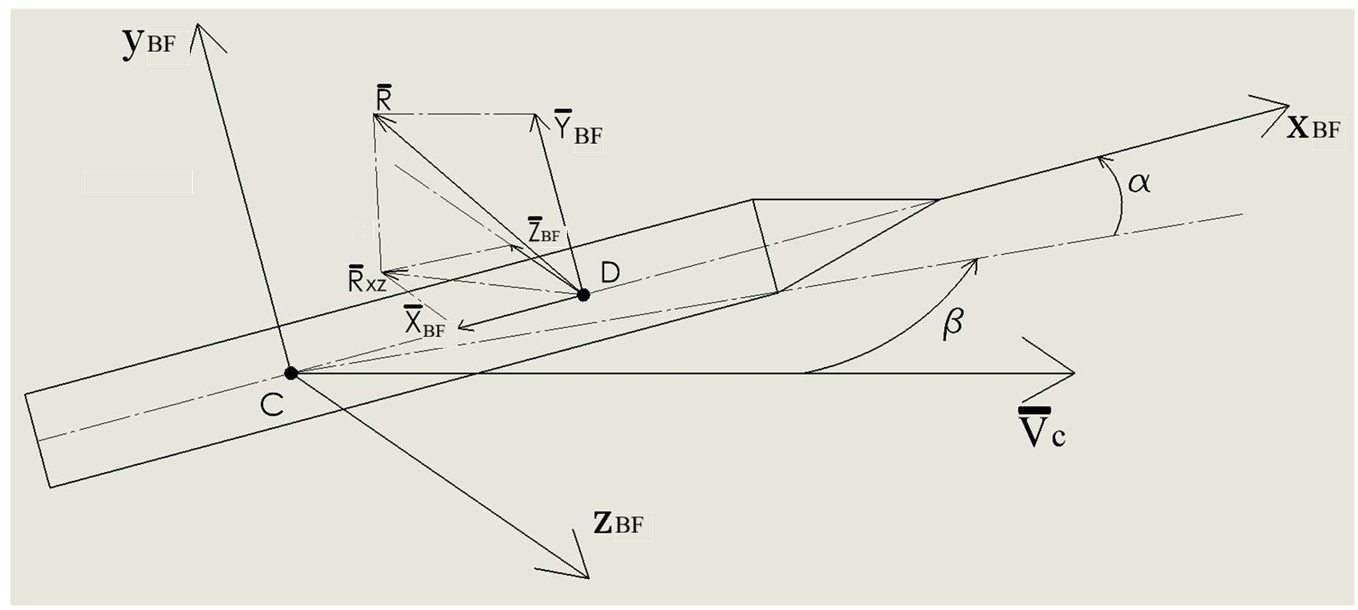
\includegraphics[width=0.6\textwidth]{BF_Sys.png}
  \caption{Body-fixed coordinate frame. The rocket is inclined relative to the velocity vector $V_c$ of the center of mass. Two angles characterise this orientation: the angle of attack $\alpha$ (between the longitudinal axis $X_b$ and the projection of $V_c$ onto the $X_b$--$Y_b$ plane) and the sideslip angle $\beta$ (between $V_c$ and the $X_b$--$Y_b$ plane). In the planar model $\beta = 0$ and only $\alpha$ is relevant. The total aerodynamic force $R$ is applied at the center of pressure $D$ and decomposed along the body axes into $X_b$, $Y_b$, $Z_b$; $R_{xz}$ denotes its projection onto the $X_b$--$Z_b$ plane. In the planar setting only $X_b$ (drag) and $Y_b$ (normal force) contribute.}
  \label{fig:bf_frame}
\end{figure}

% =============================================================================
\section{Forces and Moment}
% =============================================================================

In the body-fixed coordinate frame, the rocket experiences three aerodynamic quantities:

\begin{equation}
  \begin{cases}
    X_b = -C_x(M)\cdot\dfrac{\rho V^2}{2}\cdot S_m, & \text{[N]} \\[8pt]
    Y_b = C_y(\alpha)\cdot\dfrac{\rho V^2}{2}\cdot S_m, & \text{[N]} \\[8pt]
    M_b^z = m_z(\alpha)\cdot\dfrac{\rho V^2}{2}\cdot S_m\cdot l, & \text{[N\,m]}
  \end{cases}
\end{equation}

\begin{itemize}
  \item \textbf{$X_b$} --- drag force, directed against the velocity vector.
  \item \textbf{$Y_b$} --- normal (lift) force, arising at non-zero angle of attack.
  \item \textbf{$M_b^z$} --- pitching moment about the center of mass.
\end{itemize}

All three quantities share the same structure: a dimensionless coefficient multiplied by the dynamic pressure $q_\infty = \tfrac{1}{2}\rho V^2$ and a characteristic area $S_m$ (with an additional length $l$ for the moment).

% =============================================================================
\section{Notation}
% =============================================================================

\begin{center}
\begin{tabular}{lll}
\toprule
Symbol & Meaning & Units \\
\midrule
$C_x(M)$     & Drag coefficient (function of Mach number)        & --- \\
$C_y(\alpha)$ & Normal force coefficient (function of AoA)       & --- \\
$m_z(\alpha)$ & Pitching moment coefficient (function of AoA)    & --- \\
$\rho$        & Air density                                       & kg/m$^3$ \\
$V$           & Airspeed                                          & m/s \\
$S_m$         & Reference cross-sectional area                    & m$^2$ \\
$l$           & Reference length (rocket total length)            & m \\
$\alpha$      & Angle of attack (between rocket axis and velocity vector) & rad / deg \\
\bottomrule
\end{tabular}
\end{center}

% =============================================================================
\section{Analytical Approximations}
% =============================================================================

The dimensionless coefficients are obtained from reference tables (wind tunnel data, CFD, or empirical formulas). For the project, we use the following analytical fits, valid in two velocity regimes.

\subsection{Drag Force Coefficient}

In the low-speed incompressible regime (Mach $< 0.3$), $C_x$ is independent of Mach number and angle of attack:

\begin{equation}
  C_x = 0.358
\end{equation}

\begin{figure}[h]
  \centering
  
\includegraphics[width=0.65\textwidth]{Cx.png}
  \caption{Drag coefficient $C_x$ as a function of Mach number. In the incompressible regime (Mach $< 0.3$) the value is constant at 0.358.}
  \label{fig:cx}
\end{figure}

\subsection{Normal Force Coefficient}

\begin{equation}
  C_y(\alpha) =
  \begin{cases}
    0.05403\cdot\alpha, & V \in [0,\,500]\ \text{m/s}, \\[4pt]
    0.02599\cdot\alpha + 0.008257\cdot\alpha^2, & V \in [500,\,2200]\ \text{m/s},
  \end{cases}
\end{equation}

\begin{figure}[h]
  \centering
  
\includegraphics[width=0.65\textwidth]{Cy.png}
  \caption{Normal force coefficient $C_y(\alpha)$. The linear branch applies throughout the low-speed regime.}
  \label{fig:cy}
\end{figure}

\subsection{Pitching Moment Coefficient}

\begin{equation}
  m_z(\alpha) =
  \begin{cases}
    0.01840\cdot\alpha, & V \in [0,\,500]\ \text{m/s}, \\[4pt]
    0.02113\cdot\alpha - 0.0006463\cdot\alpha^2, & V \in [500,\,2200]\ \text{m/s},
  \end{cases}
\end{equation}

\begin{figure}[h]
  \centering
  
\includegraphics[width=0.65\textwidth]{mz.png}
  \caption{Pitching moment coefficient $m_z(\alpha)$. In the low-speed regime the dependence is strictly linear.}
  \label{fig:mz}
\end{figure}

where $\alpha$ is expressed in \textbf{degrees}.

The linear formulas (first branch) are valid throughout the incompressible regime $V \in [0, 500]$ m/s. At low speeds (Mach $< 0.3$, i.e., $V < 102$ m/s under standard conditions) thin-airfoil theory predicts linear dependence of lift and moment on angle of attack, so no separate formula is needed for $V < 100$ m/s --- the same linear coefficients apply.

% =============================================================================
\section{Operating Regime}
% =============================================================================

This project considers low-altitude flight at standard atmospheric conditions ($\rho = 1.225$ kg/m$^3$) and airspeeds up to $V \leq 100$ m/s. In this regime:

\begin{itemize}
  \item Mach number $M < 0.3$ (incompressible flow). Compressibility corrections are negligible and $C_x$ is constant.
  \item The pitching moment approximation is \textbf{strictly linear}: $m_z(\alpha) = C_{m\alpha}\cdot\alpha$ (with $\alpha$ in degrees).
  \item The proportionality coefficient
  \[
    C_{m\alpha} = 0.01840\ \text{deg}^{-1} \approx 1.054\ \text{rad}^{-1}
  \]
  is a \textbf{physical constant} of the rocket in this regime, independent of airspeed or angle of attack magnitude.
\end{itemize}

This constant $C_{m\alpha}$ appears only in the rotational dynamics --- specifically in the pitching moment term $f_2 = C_{m\alpha}\,\alpha\,q_\infty S_m l / J$ that the backstepping controller cancels exactly in the Step 3 virtual control (VC2). The translational coefficients $C_x$ and $C_{y\alpha}$ affect $(x, y)$ motion only and enter the translational equations of motion as bounded disturbances.

% =============================================================================
\section{Frame Transformation: Body-Fixed to Inertial}
% =============================================================================

The aerodynamic forces are computed in the body-fixed frame (along $X_b$ and $Y_b$ axes), but the equations of motion for the center of mass are written in the \textbf{inertial frame}. A rotation by the pitch angle $\vartheta$ converts vectors between the two frames.

\subsection{Geometry of the Transformation}

The pitch angle $\vartheta$ is measured from the vertical (inertial $y$) axis to the rocket's longitudinal axis $X_b$, with positive values corresponding to a rightward tilt. As a result:

\begin{itemize}
  \item The body axis $X_b$ is aligned with the inertial direction $(\sin\vartheta,\ \cos\vartheta)$.
  \item The body axis $Y_b$ is aligned with the inertial direction $(\cos\vartheta,\ -\sin\vartheta)$.
\end{itemize}

\subsection{Rotation Matrix}

For any vector $\mathbf{F}_{\mathrm{BF}} = (F_{X_b},\, F_{Y_b})^T$ expressed in the body frame, the corresponding inertial-frame components are:

\begin{equation}
  \begin{pmatrix} F_x \\ F_y \end{pmatrix}
  =
  \underbrace{\begin{pmatrix} \sin\vartheta & \cos\vartheta \\ \cos\vartheta & -\sin\vartheta \end{pmatrix}}_{R(\vartheta)}
  \begin{pmatrix} F_{X_b} \\ F_{Y_b} \end{pmatrix}
\end{equation}

In component form:

\begin{align}
  F_x &= F_{X_b}\sin\vartheta + F_{Y_b}\cos\vartheta, \\
  F_y &= F_{X_b}\cos\vartheta - F_{Y_b}\sin\vartheta.
\end{align}

The aerodynamic forces $(X_b, Y_b)$ computed in the body frame are substituted into the inertial-frame equations of motion using the rotation above. The pitching moment $M_b^z$ acts about the $Z_b$ axis and enters the rotational dynamics directly without requiring a frame rotation.

\bigskip
All aerodynamic forces and the regressor $Y(\alpha) = q_\infty S_m l\,\alpha$ scale proportionally with the product $S_m\cdot l$. This value must be \textbf{consistent across the simulator, the controller, and all formula evaluations}.

\end{document}
